% =====================================================
\chapter{Perceptually Guided Atmospheric Style Transfer}
\label{chap:adaptive_proposed}

This chapter presents the two adaptive systems developed in this work to push the boundaries of diffusion-based atmospheric style transfer.
InstantStyle-Plus extends the IP-Adapter framework with spatial ControlNet conditioning to enforce depth-dependent atmospheric structure; the proposed method --- \textbf{V0 (InstantStyle with CSD Guidance)} --- adds an active latent-correction loop that steers each denoising step toward the reference atmospheric style.
Both systems address the core failure identified in Chapter~\ref{chap:foundations_existing}: that unconstrained style injection changes surface appearance but not the physically coherent, depth-dependent scattering that distinguishes real atmospheric imagery.
A comparative analysis across all five evaluated methods --- StyleShot, CSGO, InstantStyle, InstantStyle-Plus, and V0 --- follows, using CLIP confidence as the primary measure of feature-space domain shift.
The central finding of this chapter is that despite clear improvements in visual realism, all four baseline methods and even V0 fail to shift the deep feature representations that large pretrained encoders rely on, motivating the physics-grounded synthesis pipeline of Chapter~\ref{chap:phase2_pipeline}.

% =====================================================
\section{InstantStyle-Plus: Spatial Conditioning for Atmospheric Style}
\label{sec:instantstyleplus}

\noindent
While InstantStyle~\cite{wang2024instantstyle} achieved strong physical realism and semantic preservation, it lacked explicit spatial control.
The model relied purely on semantic--style correspondence in latent space, which limited its ability to handle large-scale environmental transformations where geometric consistency and volumetric layering matter --- for instance, fog density varying with depth, or underwater turbidity fading toward the background.
To achieve controllable, geometry-aware, and perceptually stable stylisation under extreme environmental conditions, \textbf{InstantStyle-Plus}~\cite{wang2024instantstyleplus} was introduced.
This framework augments InstantStyle with ControlNet-based spatial conditioning and semantic adapters that maintain structural consistency and style balance during diffusion.

% -------------------------------------------------------
\subsection{Architecture and Design Motivation}
\label{sec:isp_arch}

InstantStyle-Plus builds directly upon the SDXL diffusion backbone but enhances it with three lightweight, optimisation-free modules that operate plug-and-play during inference:

\begin{itemize}
    \item \textbf{Image Adapter (IP-Adapter)~\cite{ye2023ipadapterfidelityadapters}:} aligns global semantics between the prompt and reference image using a CLIP-based projection head. This ensures that stylistic cues remain contextually relevant to the prompt semantics.
    \item \textbf{Tile ControlNet~\cite{zhang2023controlnet}:} introduces low-frequency spatial priors such as structure, edge layout, and depth hints. Through additive injection into the U-Net's up-blocks, it enforces geometric stability and prevents style overreach.
    \item \textbf{Contrastive Style Descriptor (CSD)~\cite{somepalli2024csd}:} acts as a perceptual monitor. It measures style similarity between the generated and reference images at runtime, providing non-parametric feedback to stabilise tone and texture distribution.
\end{itemize}

\noindent The SDXL~\cite{podell2023sdxlimprovinglatentdiffusion} U-Net~\cite{ronneberger2015unet} itself remains frozen; these adapters modulate its intermediate features without gradient updates, allowing real-time inference and minimal memory overhead.
At every denoising step $t$, the U-Net processes latent variables $x_t$ along with textual and visual conditioning:
\begin{equation}
    F_t = \mathrm{UNet}\!\left(x_t,\,t \;\Big|\; E_\mathrm{text}(y),\; E_\mathrm{img}(x_s),\; \mathrm{CN}_\mathrm{tile}(x_c)\right),
    \label{eq:isp_conditioning}
\end{equation}
where $E_\mathrm{text}(y)$ represents semantic embeddings from CLIP's text tower, $E_\mathrm{img}(x_s)$ the visual embeddings from the IP-Adapter, and $\mathrm{CN}_\mathrm{tile}(x_c)$ the ControlNet feature maps.
In the original image-to-image setup, $x_c$ denotes a content image that preserves layout; however, for this adaptation, it was replaced with the style reference itself, leveraging the assumption that environmental conditions implicitly encode both tone and coarse structure.

\begin{figure}[!h]
    \centering
    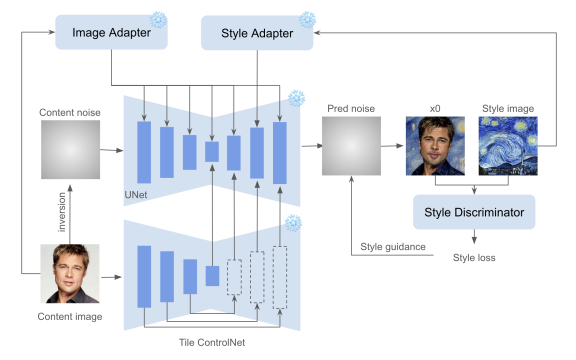
\includegraphics[width=0.65\linewidth]{images/instantstyleplus_architecture.png}
    \caption{Architecture of InstantStyle-Plus: SDXL backbone with IP-Adapter for style encoding, Tile ControlNet for spatial layout, and a frozen CSD branch for perceptual feedback (adapted from Wang et al., 2024~\cite{wang2024instantstyleplus}).}
    \label{fig:instantstyleplus_architecture}
\end{figure}

\noindent This design allows InstantStyle-Plus to treat environmental style (fog, snow, underwater hue) not merely as an artistic colour grade but as a semi-physical phenomenon tied to spatial depth and diffusion of light.
The Image Adapter ensures that the injected style remains semantically aligned with the textual intent, while the ControlNet~\cite{zhang2023controlnet} anchors the diffusion to plausible geometric contours.
The CSD~\cite{somepalli2024csd} branch, though frozen, acts as a perceptual constraint that keeps the style faithful to the reference and prevents texture drift over long denoising schedules.

% -------------------------------------------------------
\subsection{Adapted Conditioning Flow}
\label{sec:isp_conditioning}

\noindent Since the curated dataset did not include explicit content images or structural maps, InstantStyle-Plus was reconfigured into a \textbf{text + style} setup.
In this adapted configuration, the \emph{style image itself} was reused as a pseudo-content reference.
This approach stems from the observation that environmental style often carries implicit structural statistics --- fog gradients align with perspective depth, underwater absorption varies with distance, and snow blizzard streaks follow camera orientation.

\noindent Thus, both the IP-Adapter and Tile ControlNet were conditioned on the same style reference:
\begin{equation}
    \mathrm{Cond}_\mathrm{adapted} = \left\{ \mathrm{IP}_\mathrm{style}(x_s),\;\mathrm{CN}_\mathrm{tile}(x_s),\;E_\mathrm{text}(y) \right\}.
    \label{eq:isp_adapted}
\end{equation}
The IP-Adapter encodes fine tonal cues such as haze saturation, colour bias, and contrast softness; the ControlNet enforces low-frequency geometry and layout consistency; and the text encoder ensures semantic grounding in the prompt.

\noindent Meanwhile, the frozen CSD~\cite{somepalli2024csd} head periodically computes a cosine similarity between descriptor vectors of the intermediate sample $\hat{x}_t$ and the style image $x_s$, acting as a perceptual tether.
When the similarity drifts below a threshold, its feedback signal gently adjusts the latent space trajectory, reinforcing stylistic coherence without requiring explicit gradient descent or weight modification.

\begin{figure}[!h]
    \centering
    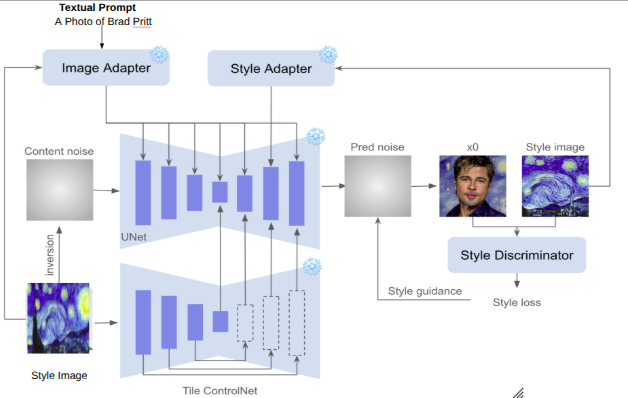
\includegraphics[width=0.92\linewidth, height=0.42\textheight, keepaspectratio]{images/instantstyleplus_flow.png}
    \caption{Adapted conditioning flow: the same style image acts as both structural and stylistic input; text embeddings guide semantics while ControlNet ensures depth-consistent spatial cues.}
    \label{fig:instantstyleplus_flow}
\end{figure}

\noindent This combined conditioning results in a richer and more interpretable diffusion process.
Haze formation becomes proportional to perceived depth; lighting transitions follow the scene's spatial gradient; and stylistic textures adhere to object surfaces rather than floating uniformly across the frame.
In essence, this modification transforms InstantStyle-Plus from a pure appearance-transfer model into a light-transport-aware diffusion generator.

% -------------------------------------------------------
\subsection{Results}
\label{sec:isp_results}

\noindent The adapted InstantStyle-Plus~\cite{wang2024instantstyleplus} produced visually richer and more spatially coherent stylisations than any prior baseline.
Spatial cues from the Tile ControlNet introduced smooth depth gradients, enabling fog and haze to appear denser at greater distances and lighter in the foreground.
The IP-Adapter preserved prompt semantics so that the environmental tone (fog, underwater, blizzard) did not overpower the subject matter.
In agricultural scenes, machinery and fencing retained shape and edge clarity while being partially enveloped by haze; underwater samples exhibited realistic blue-green attenuation and caustic diffusion around surfaces.

\noindent Quantitatively, the CLIP ViT-L/14 mean confidence --- the primary domain-shift metric used throughout this thesis --- was \textbf{0.698} for InstantStyle-Plus, substantially \emph{higher} than even the clean CIFAR-10 baseline of 0.341.
This is the pivotal finding: despite strong visual realism, the high CLIP confidence reveals that deep semantic representations are largely unchanged.
The style injection convincingly alters surface textures and colour distribution, but it does not displace the high-level feature manifold that large pretrained encoders operate on.

\begin{figure}[!h]
    \centering
    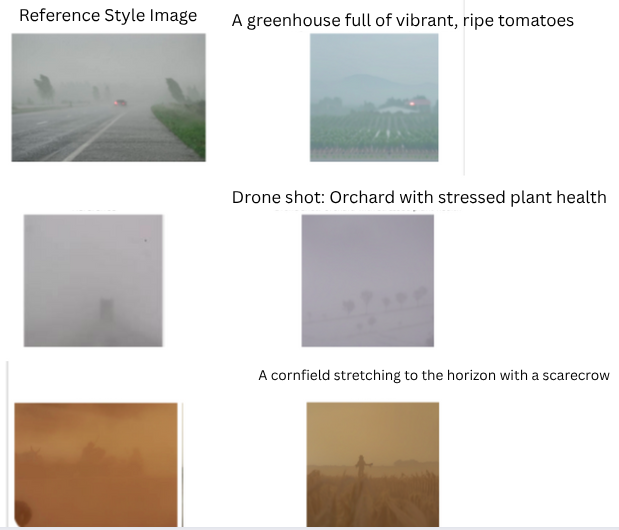
\includegraphics[width=0.8\linewidth]{images/instantstyleplus_results.png}
    \caption{Adapted InstantStyle-Plus results on the agriculture domain: improved spatial coherence and depth-consistent haze compared to plain InstantStyle. Despite strong visual quality, the CLIP ViT-L/14 confidence of 0.698 exceeds the clean-image baseline (0.341), confirming that deep feature representations are not genuinely displaced.}
    \label{fig:instantstyleplus_results}
\end{figure}

\noindent The divergence between the two metrics exposes the core limitation of appearance-based style injection.
ControlNet successfully imposes geometric consistency and depth-proportional haze density, but these are surface-level transformations.
Large vision--language encoders respond primarily to structural and semantic content, which style injection leaves intact.
Despite its improved visual realism, InstantStyle-Plus does not produce a distribution shift that would challenge a robust encoder --- and is therefore insufficient as a domain-adaptation data synthesis tool on its own.

% =====================================================
\section{V0: InstantStyle with CSD Guidance}
\label{sec:proposed_csd}

\noindent Building upon the adaptive InstantStyle-Plus, the \textbf{V0} framework integrates a lightweight \textbf{Contrastive Style Descriptor (CSD)~\cite{somepalli2024csd}} guidance loop within the InstantStyle pipeline.
The objective is to achieve continuous perceptual alignment between generated samples and the reference style image during diffusion, producing physically realistic stylisation without retraining or parameter expansion.

% -------------------------------------------------------
\subsection{Architecture}
\label{sec:prop_arch}

\noindent V0 retains the SDXL diffusion backbone and the IP-Adapter for style conditioning.
CSD acts as a frozen perceptual critic that evaluates intermediate generations during inference and slightly adjusts the diffusion latents to maintain style alignment.

\textbf{Core Components:}
\begin{itemize}
    \item \textbf{SDXL~\cite{podell2023sdxlimprovinglatentdiffusion} Backbone:} provides the denoising foundation and latent diffusion process. The U-Net remains fully frozen.
    \item \textbf{IP-Adapter~\cite{ye2023ipadapterfidelityadapters} with block-selective injection:} extracts a style embedding from the reference image via CLIP ViT-H/14 and injects it through cross-attention into the final up-blocks of the U-Net (\texttt{up\_blocks.0.attentions.1} and \texttt{up\_blocks.1}), with all other blocks zeroed.
    \item \textbf{CSD Module~\cite{somepalli2024csd}:} a frozen ViT-L/14 encoder fine-tuned for style similarity that computes normalised style descriptors, enforcing perceptual consistency between intermediate generations and the reference.
\end{itemize}

\begin{figure}[htbp]
    \centering
    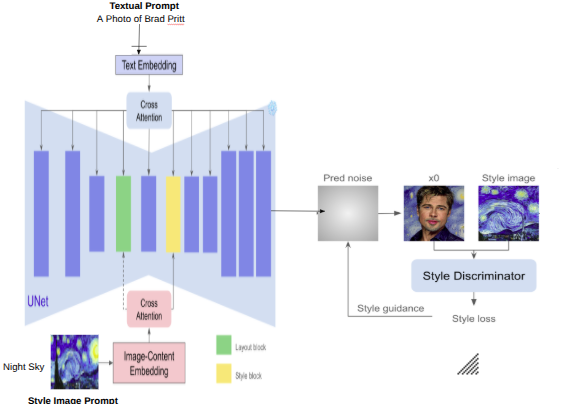
\includegraphics[width=0.97\linewidth]{images/proposed_architecture.png}
    \caption{V0 architecture: SDXL U-Net backbone with IP-Adapter for style conditioning and a frozen CSD module that periodically evaluates perceptual similarity between the partially decoded generation and the reference atmospheric image, adjusting the latent direction to enforce style alignment (adapted from Wang et al., 2024~\cite{wang2024instantstyle}).}
    \label{fig:v0_architecture}
\end{figure}

% -------------------------------------------------------
\subsection{CSD Guidance Loop}
\label{sec:csd_loop}

\noindent At selected timesteps (every third denoising step), the partially denoised image $\hat{x}_t$ is decoded and passed through the CSD network to obtain an embedding $s(\hat{x}_t)$.
The cosine similarity with the reference descriptor $s(x_\mathrm{ref})$ defines the perceptual loss:
\begin{align}
    \mathcal{L}_\mathrm{CSD} &= -\,\cos\!\bigl(\mathrm{CSD}(\hat{x}_t),\; \mathrm{CSD}(x_\mathrm{ref})\bigr), \label{eq:csd_loss} \\
    z_t &\leftarrow z_t - \eta \cdot \frac{\nabla_{z_t}\mathcal{L}_\mathrm{CSD}}{\left\|\nabla_{z_t}\mathcal{L}_\mathrm{CSD}\right\|} \cdot \sigma(z_t), \label{eq:csd_update}
\end{align}
where $z_t$ is the current diffusion latent and $\eta=0.16$ is a small correction step.
The normalisation of the gradient vector ensures correction magnitude is stable regardless of loss curvature; $\sigma(z_t)$ scales the correction proportionally to current noise level.

\noindent This integration is entirely parameter-free and all model weights remain frozen.
The CSD~\cite{somepalli2024csd} operates externally as a perceptual evaluator, guiding generation through latent corrections rather than retraining.
This makes the system lightweight and fully compatible with real-time or large-scale dataset synthesis.

% -------------------------------------------------------
\subsection{Experimental Setup}
\label{sec:prop_exp}

\noindent Experiments were conducted on the same curated 500-image benchmark covering fog, snow, storm, sand/dust, and underwater conditions.
All runs used:
\begin{itemize}
    \item Resolution: $896\times896$ pixels.
    \item Denoising steps: 40 (DDIM scheduler).
    \item Guidance scale: 3.6 (classifier-free guidance).
    \item CSD feedback: every 3 steps, $\eta=0.16$.
    \item Style injection: \texttt{up\_blocks.0} and \texttt{up\_blocks.1} only (IP-Adapter scale 1.0).
    \item 5 agricultural content prompts $\times$ 5 random seeds = 25 runs per style domain.
\end{itemize}
No auxiliary priors (for example, fog bias) were used; negative prompts excluded anti-blur terms, enabling natural haze formation.

% -------------------------------------------------------
\subsection{Results}
\label{sec:prop_results}

\noindent Qualitatively, V0 produced the most visually consistent stylisations among all evaluated style transfer methods.
Haze scenes displayed smooth depth-dependent fading; blizzards and sandstorms produced realistic occlusion and tonal balance; underwater domains showed wavelength-dependent colour absorption and subtle backscatter.
Edges softened naturally with distance, producing volumetric haze around subjects.
CSD feedback stabilised tone transitions across denoising steps and suppressed overexposure in high-luminance regions.

\noindent Quantitatively, the CLIP ViT-L/14 confidence was \textbf{0.514} and the CLIP ViT-H/14 confidence was \textbf{0.438}.
This is the strongest result in the style transfer study --- the lowest confidence of any evaluated style-transfer method --- yet both values remain above the clean baseline (ViT-L: 0.341, ViT-H: 0.335), and well above the physics pipeline V3's 0.274 and 0.246 respectively.
CSD guidance measurably pulls latent representations toward the style reference's feature space, but it cannot overcome the generative model's prior, which preserves semantic structure by design.
The CSD guidance loop introduces a mild but measurable pull toward the style reference's feature distribution, but it cannot compensate for the fundamental limitation of latent-space style injection: the diffusion model generates images that look atmospheric, yet the generative prior keeps semantic content intact.

\begin{figure}[!h]
    \centering
    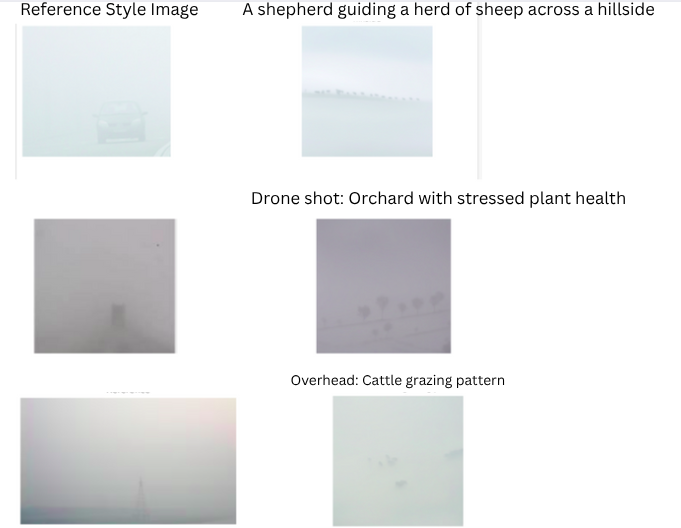
\includegraphics[width=0.8\linewidth]{images/proposed_results.png}
    \caption{V0 (InstantStyle~\cite{wang2024instantstyle} + CSD~\cite{somepalli2024csd} Guidance) on the agriculture domain: enhanced depth-aware haze and stable tone. CLIP ViT-L/14 confidence 0.514 and ViT-H/14 confidence 0.438 --- the lowest of all evaluated style transfer methods, yet still above the clean baseline, and a substantial gap remains to the V3 physics pipeline (0.274 / 0.246).}
    \label{fig:proposed_results}
\end{figure}

\noindent The CSD guidance loop acts as a non-trainable perceptual critic, applying latent corrections every third denoising step with minimal inference overhead ($<5\%$).
Despite being the strongest result in the style transfer study, it confirms that perceptual contrastive feedback alone cannot close the gap between appearance-based synthesis and physics-grounded distribution shift.
Ablating the CSD guidance (setting $\eta=0$) reverted results to baseline InstantStyle levels, confirming the contribution is real --- but the ceiling imposed by style injection itself remains the binding constraint.

% =====================================================
\section{Comparative Analysis}
\label{sec:qualitative_comparison}

\noindent This section summarises the comparative results across all five evaluated models --- StyleShot~\cite{gao2024styleshot}, CSGO~\cite{xing2024csgocomp}, InstantStyle~\cite{wang2024instantstyle}, InstantStyle-Plus~\cite{wang2024instantstyleplus}, and V0 (InstantStyle + CSD Guidance) --- using both qualitative and quantitative indicators.
The goal was not to maximise classification accuracy but to assess the \textbf{extent and realism of distribution-shift generation} under adverse environmental styles.

% -------------------------------------------------------
\subsection{Qualitative Comparison}
\label{sec:qualitative_grid}

Representative outputs from the curated dataset are shown in Figure~\ref{fig:qualitative_grid}.
Across five reference prompts (\textit{tractor ploughing field}, \textit{cornfield horizon}, \textit{sheep herd}, \textit{greenhouse}, and \textit{flooded crop area}), the progressive improvement in visual realism and depth consistency is clearly visible.

\begin{figure}[htbp]
    \centering
    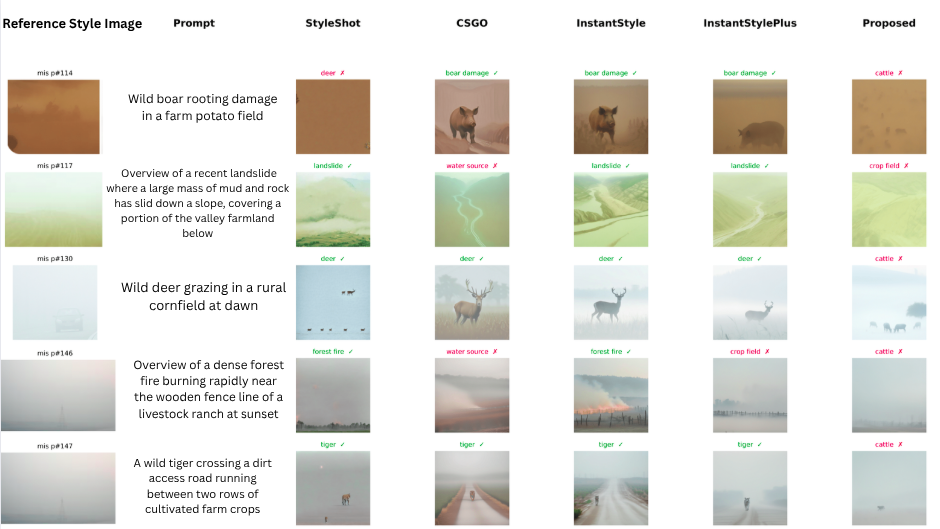
\includegraphics[width=\textwidth, height=0.9\textheight, keepaspectratio]{images/final_all_grid.png}
    \caption{Qualitative comparison (five representative samples) across StyleShot, CSGO, InstantStyle, InstantStyle-Plus, and V0. V0 achieves realistic environmental veiling and depth-consistent haze while preserving semantic integrity.}
    \label{fig:qualitative_grid}
\end{figure}

\noindent\textbf{Observations:}
\begin{itemize}
    \item \textbf{StyleShot~\cite{gao2024styleshot}:} Produced overly artistic and painterly generations. While visually appealing, it performed poorly at style transfer, merely recolouring the scene without volumetric haze or realistic scattering. The model lacks depth-aware modulation, making its outputs aesthetically strong but physically implausible.
    \item \textbf{CSGO~\cite{xing2024csgocomp}:} Improved overall tonal blending but still lacked volumetric realism. Edges remained unnaturally sharp, and atmospheric style appeared as global filters rather than media that wrap around objects.
    \item \textbf{InstantStyle~\cite{wang2024instantstyle}:} Delivered the most balanced realism among existing systems, achieving physically faithful haze and turbidity while preserving prompt semantics and stable colour consistency.
    \item \textbf{InstantStyle-Plus~\cite{wang2024instantstyleplus}:} Enhanced spatial and semantic stability through ControlNet~\cite{zhang2023controlnet} integration, creating smoother volumetric cues and reducing chromatic drift, though sometimes slightly softening contrast.
    \item \textbf{V0 (InstantStyle + CSD Guidance):} Combined all strengths --- strong volumetric realism, perceptually coherent tone alignment, and stable structure --- with minimal added computation.
\end{itemize}

\FloatBarrier
% -------------------------------------------------------
\subsection{Quantitative Evaluation}
\label{sec:quantitative_results}

\noindent Table~\ref{tab:phase1_accuracy} reports CLIP confidence for all five methods using ViT-L-14 and ViT-H-14 (metaclip\_fullcc) --- the same backbone family used in the physics-grounded pipeline --- enabling a consistent cross-method comparison.
Confidence (mean max-softmax score over 100 ImageNet classes) is the primary domain-shift metric throughout this thesis: lower confidence means the image has moved further from the clean-image distribution that CLIP was trained to recognise.

\begin{table}[!h]
\centering
\caption{Style transfer evaluation: CLIP ViT-L-14 and ViT-H-14 (metaclip\_fullcc) confidence and top-1 accuracy on style-transferred outputs (60 images per method, same 15 agricultural prompts as the physics-grounded pipeline). Lower confidence = stronger distribution displacement. Top-1 accuracy measures whether the agricultural scene label is still recognisable; a drop here signals semantic corruption rather than genuine domain shift.}
\label{tab:phase1_accuracy}
\resizebox{\textwidth}{!}{%
\renewcommand{\arraystretch}{1.3}
\setlength{\tabcolsep}{5pt}
\begin{tabular}{lcccc}
\toprule
 & \multicolumn{2}{c}{\textbf{CLIP ViT-L-14}} & \multicolumn{2}{c}{\textbf{CLIP ViT-H-14}} \\
\cmidrule(lr){2-3}\cmidrule(lr){4-5}
\textbf{Method} & \textbf{Conf.\ ($\downarrow$)} & \textbf{Top-1 (\%, $\uparrow$)} & \textbf{Conf.\ ($\downarrow$)} & \textbf{Top-1 (\%, $\uparrow$)} \\
\midrule
InstantStyle~\cite{wang2024instantstyle}            & 0.661 & 84.4 & 0.652 & 75.0 \\
InstantStyle-Plus~\cite{wang2024instantstyleplus}   & 0.698 & 80.32 & 0.659 & 76.43 \\
StyleShot~\cite{gao2024styleshot}                   & 0.620 & 56.2 & 0.552 & 65.6 \\
CSGO~\cite{xing2024csgocomp}                        & 0.625 & 87.5 & 0.587 & 81.2 \\
\textbf{V0 (InstantStyle + CSD)}              & \textbf{0.514} & \textbf{76.43} & \textbf{0.438} & \textbf{74.78} \\
\midrule
\textit{Clean baseline}                             & \textit{0.341} & \textit{---}    & \textit{0.335} & \textit{---} \\
\textit{V3 Physics Pipeline (reference)}             & \textit{0.274} & \textit{67.2} & \textit{0.246} & \textit{67.4} \\
\bottomrule
\end{tabular}
}
\end{table}

\noindent The confidence column is the decisive finding.
Four of the five evaluated style transfer methods --- InstantStyle (0.661), InstantStyle-Plus (0.698), StyleShot (0.620), and CSGO (0.625) --- have CLIP ViT-L/14 confidence \emph{above} the clean baseline of 0.341, meaning style injection leaves deep representations largely intact.
V0 achieves the lowest confidence among all style transfer methods at 0.514 (ViT-L/14) and 0.438 (ViT-H/14), confirming that CSD guidance does measurably push representations away from the clean-image manifold.
However, both values remain \emph{above} the clean baseline (0.341 / 0.335) --- appearance-based style injection cannot cross this threshold regardless of how sophisticated the guidance loop is.
The V3 physics pipeline achieves 0.274/0.246, well below both clean baselines.

\noindent The top-1 accuracy column ($\uparrow$ desirable: higher means the agricultural scene label is still recognisable, confirming semantic integrity) shows a consistent picture.
V0 retains high accuracy (76.43\% / 74.78\%), meaning the images are visually atmospheric but semantically unchanged --- CLIP readily recovers the original class through the style overlay.
The V3 physics pipeline achieves 67.2\%/67.4\% --- slightly lower, because the Koschmieder physics compositor genuinely attenuates scene content with depth, introducing mild label ambiguity at high-beta settings --- while simultaneously achieving the strongest confidence drop.
This combination --- lower confidence \emph{and} maintained semantic recognisability --- is the hallmark of high-quality domain-adaptation training data, and it is unachievable through appearance-based style injection alone.

% -------------------------------------------------------
\subsection{Parameter Efficiency}
\label{sec:parameter_efficiency}

\noindent A model's practicality depends not only on realism but also on computational footprint.
Table~\ref{tab:phase1_params} summarises parameter statistics for each framework.

\begin{table}[!h]
\centering
\caption{Parameter comparison across evaluated frameworks. The proposed method retains the same lightweight footprint as InstantStyle despite adding perceptual feedback.}
\label{tab:phase1_params}
\renewcommand{\arraystretch}{1.3}
\begin{tabular}{lcc}
\toprule
\textbf{Method} & \textbf{Total Params (B)} & \textbf{Trainable (M)} \\
\midrule
StyleShot~\cite{gao2024styleshot}                   & 2.1--2.2 & 435--585 \\
CSGO~\cite{xing2024csgocomp}                        & 6.6--6.7 & 650--760 \\
InstantStyle~\cite{wang2024instantstyle}            & 6.0 & 22 \\
InstantStyle-Plus~\cite{wang2024instantstyleplus}   & 7.2--7.5 & 600--700 \\
\textbf{V0 (InstantStyle + CSD)}              & 6.6--6.7 & \textbf{22} \\
\bottomrule
\end{tabular}
\end{table}

\noindent Despite integrating perceptual feedback, the proposed method retains nearly the same parameter count as InstantStyle, confirming that \textbf{quality improvements stem from perceptual correction, not additional learnable modules}.
This efficiency makes it particularly suitable for real-time or low-resource generative applications.

% -------------------------------------------------------
\subsection{Insights}
\label{sec:discussion_overall}

From both qualitative and quantitative perspectives, the models reveal clear trade-offs:
\begin{itemize}
    \item \textbf{StyleShot~\cite{gao2024styleshot}:} Generates artistic stylised outputs but lacks volumetric cues. CLIP confidence (0.620) remains substantially above the clean baseline, confirming the style overlay does not shift deep feature representations.
    \item \textbf{CSGO~\cite{xing2024csgocomp}:} Provides stable tonal fusion but CLIP confidence (0.625) is similarly high. The CLIP top-1 accuracy of 87.5\% is paradoxically the highest of all methods, indicating that CSGO's style changes actually make classes \emph{more} recognisable to CLIP.
    \item \textbf{InstantStyle~\cite{wang2024instantstyle}:} CLIP ViT-L/14 confidence (0.661) is the second-highest of all methods, well above the clean baseline. Its top-1 accuracy (84.4\%) confirms that its outputs remain easily classifiable --- no genuine domain shift.
    \item \textbf{InstantStyle-Plus~\cite{wang2024instantstyleplus}:} Produces the best visual quality among existing methods. Yet its CLIP ViT-L/14 confidence (0.698) is the highest of all --- geometry-aware stylisation paradoxically makes features more classifier-friendly rather than displacing them.
    \item \textbf{V0 (InstantStyle + CSD Guidance):} The strongest result in the style transfer study: CLIP confidence 0.514 (ViT-L/14) and 0.438 (ViT-H/14), the lowest of all evaluated style transfer methods. CSD feedback measurably nudges generation toward the style reference's feature space, but both values remain above the clean baseline (0.341 / 0.335) --- the generative prior preserves semantic structure by design, imposing a hard ceiling on style-injection-based domain shift.
\end{itemize}

\noindent The central lesson from the style transfer study is that appearance-based style transfer and deep feature-space domain shift are not the same thing.
All evaluated style transfer methods produce images that look more atmospheric than the clean source --- but CLIP encoders, trained on billions of web images including hazy and adverse-weather scenes, readily look through the appearance change and recover the underlying semantic content.
Style injection changes the \emph{render} of an image; it does not change the \emph{information} encoded in the image.
Only physics-grounded synthesis --- where the scattering medium physically attenuates, mixes, and obscures luminance in proportion to scene depth --- disrupts the information structure that large encoders depend on.

% =====================================================
\section{Summary}
\label{sec:phase1_summary}

\noindent This chapter traced the full arc of the style transfer study: from the spatial conditioning of InstantStyle-Plus through the perceptually guided V0 system, to a comparative evaluation across all five methods.
InstantStyle-Plus demonstrated that reusing the style image as a pseudo-content reference for Tile ControlNet produces depth-consistent volumetric effects that plain style injection cannot, but its CLIP ViT-L/14 confidence (0.698) exceeded even the clean baseline (0.341), revealing that improved visual fidelity does not translate into genuine feature-space displacement.
V0 (InstantStyle + CSD Guidance) achieved the strongest result in the style transfer study --- CLIP ViT-L/14 confidence 0.514, ViT-H/14 confidence 0.438, top-1 accuracy 76.43\%/74.78\% --- but both confidence values remained above the clean baseline (0.341 / 0.335), and the gap to the V3 physics pipeline (0.274 / 0.246) remained substantial.

\noindent The core finding of the style transfer study is a negative one: four of five methods fail the CLIP confidence test entirely, and even the best method only partially crosses the clean-image boundary on the stronger encoder.
Style transfer changes how an image looks; it does not change what a large pretrained encoder sees.
The CLIP model, having been trained on internet-scale atmospheric imagery, readily recovers semantic content through stylistic surface overlays.
These findings directly motivate the physics-grounded synthesis pipeline of Chapter~\ref{chap:phase2_pipeline}, where Koschmieder-based depth compositing attenuates, mixes, and obscures luminance in proportion to scene depth --- creating a physical information barrier that appearance-based generation cannot replicate and that large encoders cannot trivially see through.
